\documentclass[landscape,12pt,openany]{book}

\usepackage{multicol}
\usepackage{tabularx}
\usepackage{graphicx}
\graphicspath{{./images/}}
\usepackage[margin=.75in, paperwidth=8.5in, paperheight=11in]{geometry}
\usepackage{titlesec}
\usepackage{xfrac}
\usepackage{mdframed}
\usepackage{gensymb}
\usepackage[abs]{overpic}
\setlength\unitlength{1in}
\usepackage{color}

\usepackage{cookbook}  % custom style

\titlespacing*{\chapter}{0em}{-3em}{1em}
\titleformat{\chapter}{\normalfont\huge\bfseries}{\chaptertitlename\
\thechapter:}{20pt}{\Huge}
\renewcommand{\thesection}{}  % don't show the section numbers
\titleformat{\section}[block]{\titlerule\scshape\large\filcenter\vspace{2pt}}{}{0em}{}[\titlerule]
\titleformat{\subsection}[block]{\scshape\large\filcenter}{}{0em}{}[\titlerule]
\setlength{\parindent}{0em}
\setlength{\columnseprule}{0.4pt}
\pagestyle{plain}
\usepackage[utf8]{inputenc}
\usepackage[T1]{fontenc}

\begin{document}

\rmfamily

\setlength{\columnseprule}{0pt}
\columnsep=2em

\setcounter{tocdepth}{1}
\small
\tableofcontents

\normalsize

\setlength{\parskip}{.5em}

\chapter{Salads}
\section{Caesar Salad}
\begin{recipe}

Place serving bowls and large mixing bowl in the freezer.

\ingredients{
    \sfrac{1}{2} & loaf rye bread \\
    \sfrac{1}{4} & cup olive oil \\
              5  & garlic cloves \\
}

Simmer smashed garlic cloves in oil for 10 minutes to flavor the oil.

Cut bread into \sfrac{1}{2} inch cubes. Spread on a baking sheet and paint with olive oil mixture.

Bake at 350\degree{} for 10 minutes, and then continue to bake, watching closely, until golden brown.

Place croûtons in an open container and put in the freezer for 10 minutes.

\ingredients{
   1 & block parmesan reggiano \\
}

Grate 1 cup coarse, and \sfrac{1}{2} cup fine.

\ingredients{
    2 & heads romaine hearts \\
}

Cut into \sfrac{3}{4} inch rounds, separate and then chop roughly.

\ingredientsLeft{
    & dressing \\
    & fresh pepper \\
}

When you're ready to serve, remove large mixing bowl from freezer. Combine lettuce, cheese, pepper and two large spoonfuls of dressing.

Add croûtons, and mix again briefly. Turn out into serving bowls from the freezer.

\subsection{Caesar Dressing}

\ingredients{
               1 & large egg \\
               3 & tablespoons lemon juice \\
               1 & teaspoon Worcestershire \\
   1\sfrac{1}{2} & teaspoon anchovy paste \\
               1 &  clove garlic \\
}

Blanch egg in shell for 45 seconds in boiling water. Remove and crack into a small bowl. Whisk with other ingredients.

\ingredients{
    \sfrac{1}{3} & cup olive oil (extra-virgin) \\
}

Slowly whisk oil into the dressing. Season to taste with salt and pepper.

\end{recipe}

\newgeometry{margin=0in}
\begin{figure}[p]
    \centering
    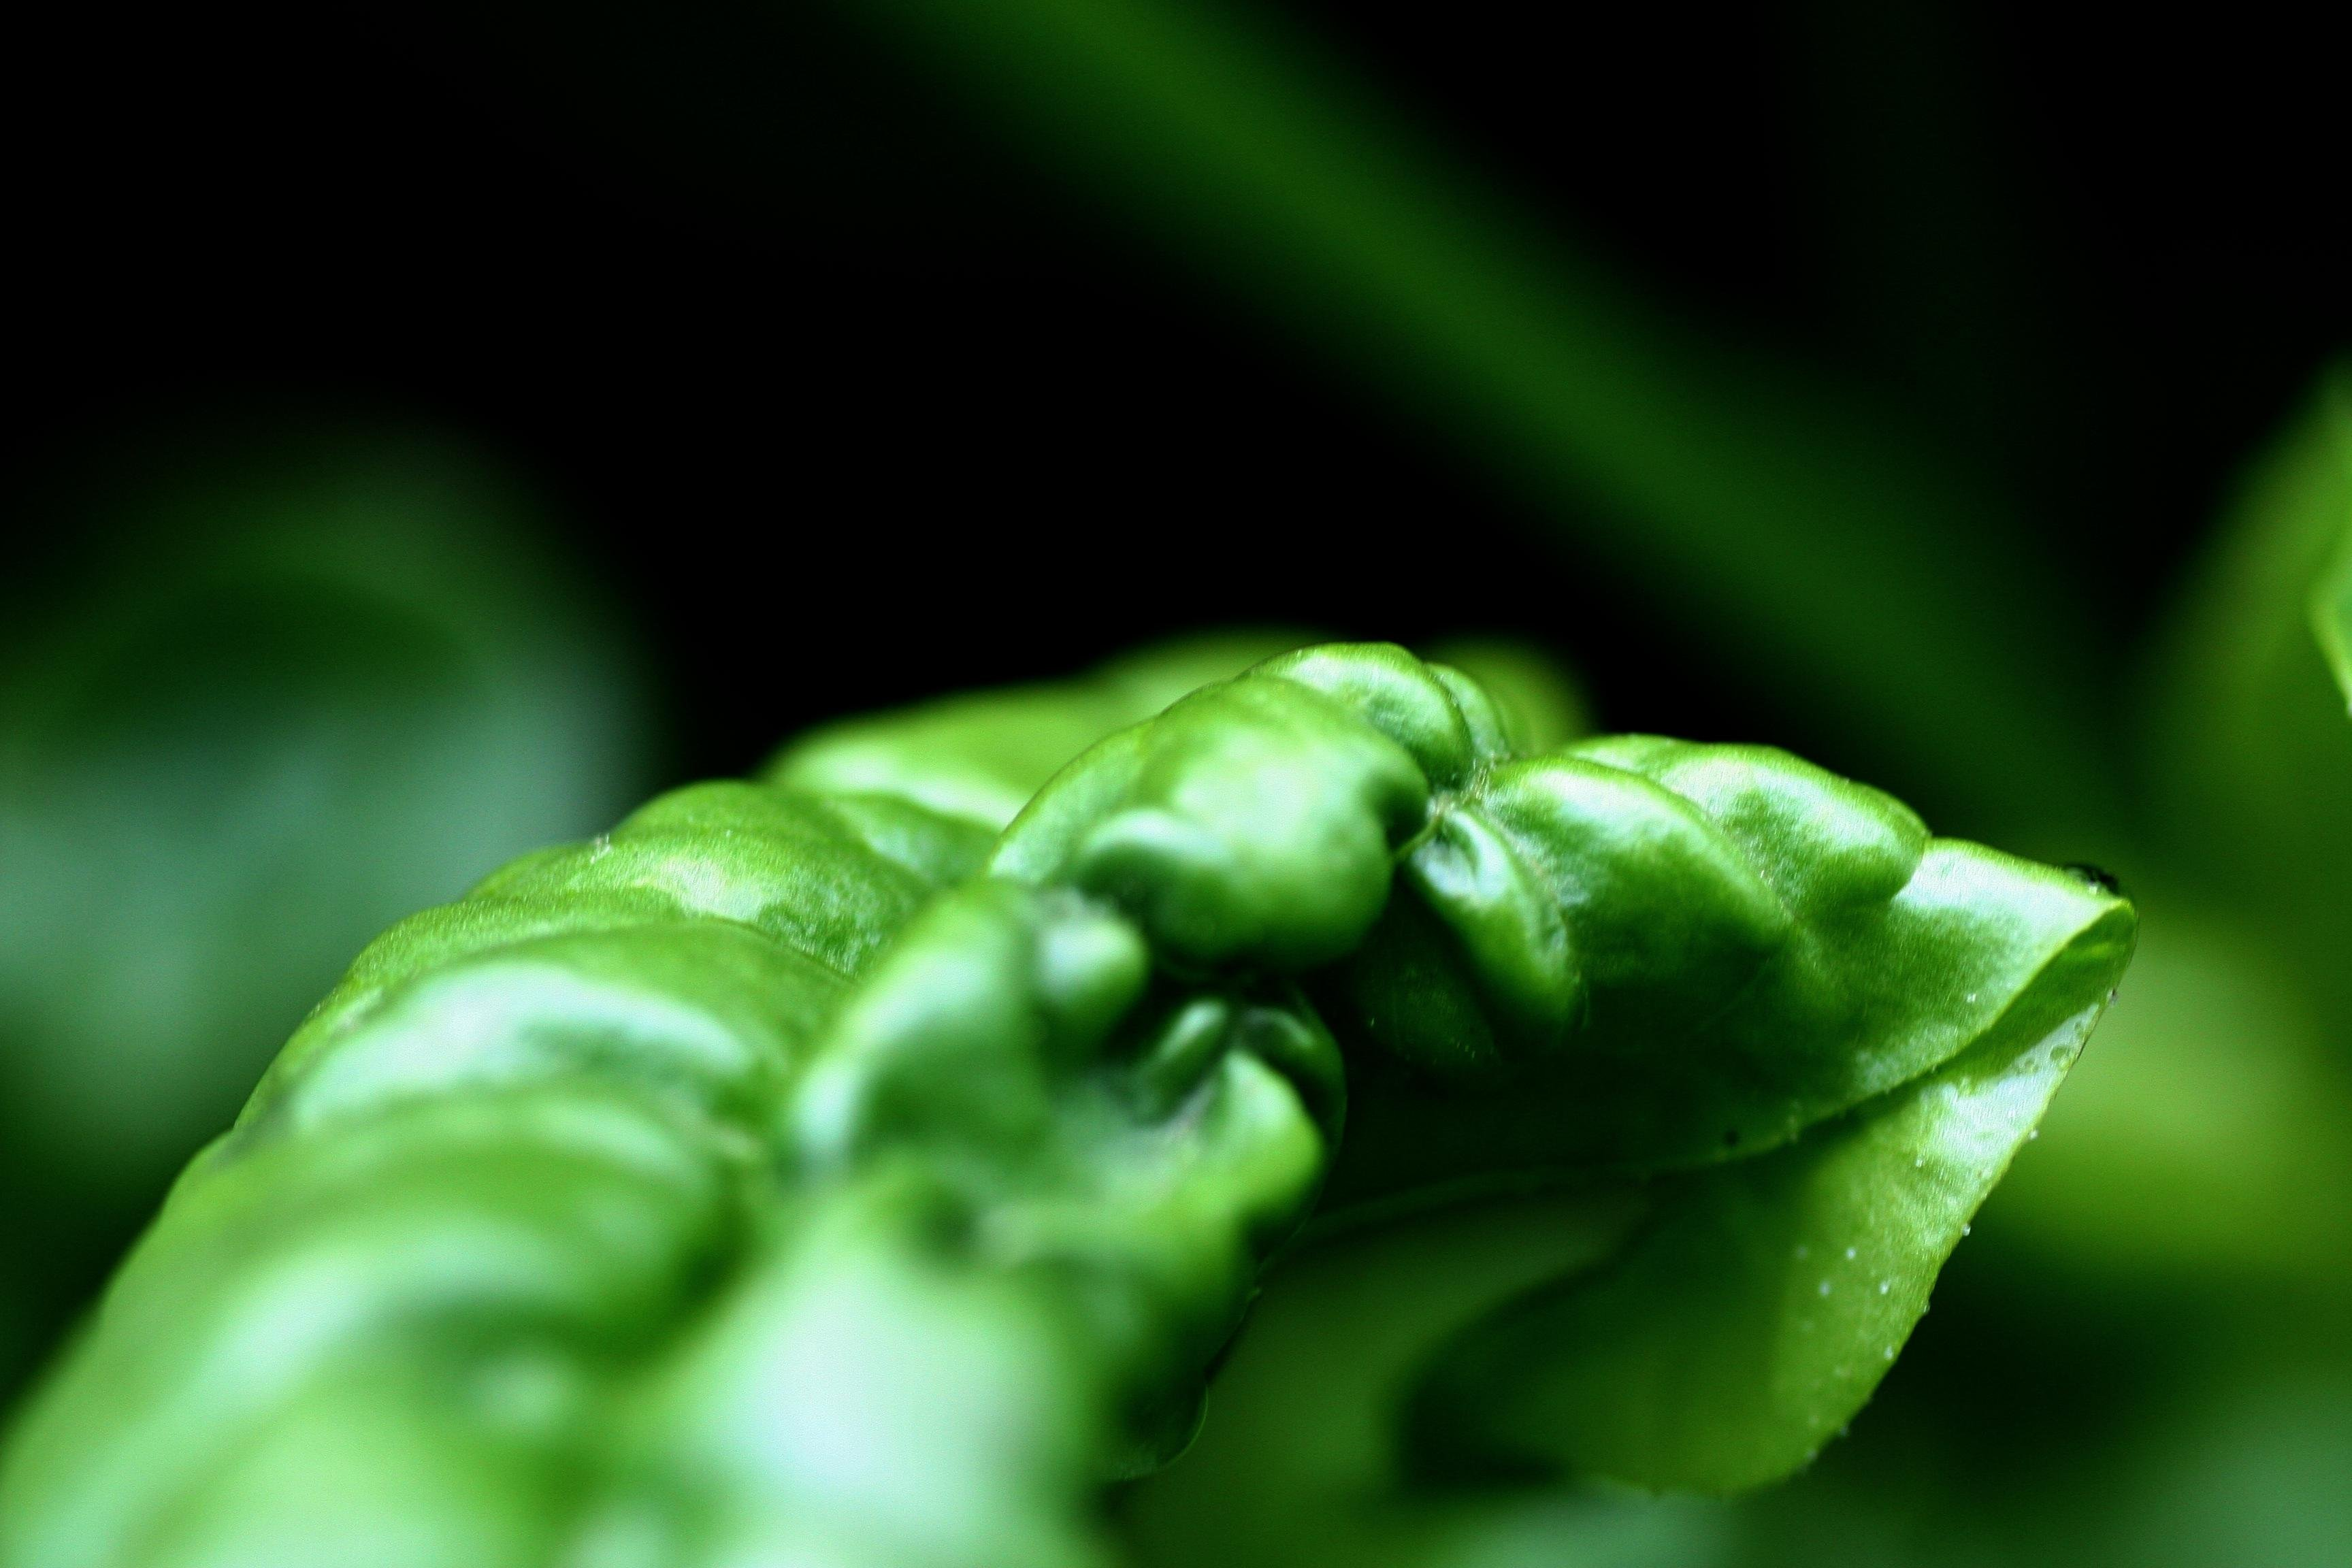
\includegraphics[width=\paperwidth,height=\paperheight]{spinach.jpg}
    \caption{Fresh Spinach}
\end{figure}
\restoregeometry
\clearpage

\section{Anne's Spinach Salad}
\begin{multicols*}{3}

\begin{quote}
    This recipe is from my Aunt Anne, who swears that she always used romaine lettuce instead of spinach.
\end{quote}

\begin{tabular}{r@{ }l}
    2 & eggs \\
\end{tabular}

Boil eggs, cool, shell and slice into rings.

\begin{tabular}{r@{ }l}
    10 & strips bacon \\
\end{tabular}

Separate strips onto aluminum foil in a baking sheet, and bake for 15 minutes at 425. Pat dry and chop into small pieces.

\begin{tabular}{r@{ }l}
    \sfrac{1}{2} & cup olive oil \\
    \sfrac{3}{4} & can anchovies in oil \\
               2 & tablespoons balsamic \\
               2 & tablespoons lemon juice \\
               1 & garlic clove \\
    \sfrac{1}{2} & teaspoon thyme \\
    \sfrac{1}{4} & teaspoon \\
                 & sugar \\
                 & oregano \\
                 & mustard powder \\
                 & onion salt \\
                 & paprika \\
\end{tabular}

Discard the oil in the can and use only the anchovies. Liquefy all  ingredients in a blender.

\begin{tabular}{r@{ }l}
    1 & package spinach \\
      & pre-sliced mushrooms \\
\end{tabular}

Combine eggs, bacon and dressing in a large mixing bowl.

\begin{quote}
The dressing can keep at least overnight.

To shell eggs easily, run under cold water, shaking pan to smash shells. The water will seep in. In 10 minutes, the shells will come off easily.

Leftover spinach can be saved, but be sure to reseal it in the original packaging, which is specially designed to breath. Spinach or lettuce saved in regular plastic will rot in a few days.

If you want to chop bacon very fine, freeze it for 10 minutes first.
\end{quote}

\end{multicols*}

\clearpage

\section{Kick-Ass Kale Salad}
\begin{recipe}

\pre{
    This salad was served by a caterer at a startup I worked for. I asked the chef about the recipe, and took copious notes so I could try to replicate it.
}

\ingredients{
    2 & heads Luciano kale \\
}

Remove the ribs of the kale by folding the leaves over lengthwise and stripping them through your curled fingers. Chop kale into ribbons of approximately \sfrac{1}{4} inch.

\ingredients{
    \sfrac{1}{2} & cup olive oil \\
    \sfrac{1}{4} & cup lemon juice \\
               2 & garlic cloves \\
}

Mince garlic and whisk ingredients together to create a vinaigrette dressing.

\ingredients{
    12 & ounces Edamame beans \\
     8 & ounces Pecorino cheese \\
       & kosher salt \\
       & pepper \\
}

\tip {
    Frozen Edamame is just fine, and so much more convenient than shelling pods. Just defrost ahead of time.
}

Grate cheese and combine ingredients in a large bowl. Season liberally with salt and pepper. Kale can take a lot of salt!

Serve with Sriracha for the adventurous.

\end{recipe}

\section{Quarantine Salad with warm Brussels and Feta}
\begin{recipe}

\tip {
    The still-warm Brussel sprouts are what make this salad. They bring out
    the flavor of the feta.
}


This recipe is for single serving. This salad can take salt and Sriracha well.

\ingredients{
       & young mixed greens (aka spring mix) \\
       \sfrac{1}{2} & cup feta cheese, small crumble \\
       & whole shelled pistachios \\
}

Mince spring mix finely. Layer lettuce, feta, and pistacios in a bowl. 

\ingredients{
       & Brussel sprouts \\
}

Slice brussel sprouts and sauté in a pan with olive oil until the leaves are blackened. 

Top salad with warm Brussel sprouts, and season to taste
with salt and Sriracha.

\end{recipe}


\fullpageimage{couscous.jpg}{http://www.flickr.com/photos/stone-soup}

\section{Couscous Salad}
\begin{recipe}

\pre{
    Couscous has a tendency to clump together. Ideally, we want every kernel to be separate. Also, you want to serve the final salad as cold as possible. That means no lukewarm couscous.
}

\ingredients{
    1 & handful kosher salt \\
    3 & trays ice cubes \\
}

In one large metal bowl, combine ice, kosher salt, and enough water to cover the ice fully.

\ingredients{
    2 & boxes plain couscous \\
    1 & tablespoon butter \\
}

Follow the directions on the box to hydrate couscous. Immediately after the couscous is cooked, turn out into another metal bowl.

\columnbreak

\ingredients{
    \sfrac{1}{2} & cup Italian dressing \\
}

Mix the dressing into the couscous to help it separate. Fluff with a spatula, breaking up as many clumps as possible.

Place the metal bowl with the couscous into the bowl with the ice. Keep stirring every three minutes to break down the clumps.

\ingredients{
                6 & ounces feta cheese \\
                1 & orange bell pepper \\
                1 & yellow bell pepper \\
     \sfrac{1}{2} & large red onion \\
}

Dice the peppers and onion fine, and combine with feta cheese in the couscous bowl.

\ingredientsLeft{
    & Italian dressing \\
    & kosher salt \\
    & pepper \\
    & dried dill \\
}

Season to taste.

\columnbreak

\tip{
    The two large metal bowls with ice water is great for cooling just about anything quickly. It's kind of like a reverse double-boiler.
}

\tip{
    The boxed Couscous sold in the grocery store is actually pre-cooked, which is why it only takes a few minutes to hydrate. You can buy uncooked Couscous, which has larger grains and cooks like pasta.
}

\tip{
    When buying feta, I prefer the cryo-packed version with a little bit of juice sealed in. The free-standing feta in juice and the Saran-wrapped versions are dryer.
}

\end{recipe}

\section{Potato Salad}
\begin{recipe}

\pre{
    The key to this potato salad is cooking and cooling the potatoes completely, before 
    cutting them up, or stirring them. Otherwise, the potatoes start to break down and 
    muddy the salad. While they are hot, you want to both salt and season them with 
    vinegar (pickle juice). If you can cook the potatoes inside a fitted colander inside 
    a large pot, then they will bairly be distrubuted while cooking or cooling. 
}

\ingredients{
    3 & pounds medium or small yukon gold potatoes \\
    4 & quarts water \\
    & kosher salt \\    
    & pickle juice \\ 
}

Heavily salt water, put potatoes in, and bring to a boil. The water does not need to 
be at a boil before you put the potatoes in. Once boiling, reduce heat to a 
medium boil. Cook for 15 to 25 minutes, or until a knife easily pierces a potato. 

Drain potatoes using a colander. Place a colander with potatoes inside a large bowl. 
Pour (strained) pickle juice over the hot potatoes. Using another large bowl, move 
colander back and forth, and continue to pour the pickle juice over the potatoes every 
minute, until they stop steaming.

Leave potatoes out at room temperature to cool completely, before cutting them. 

\ingredients{
                2 & cups mayonnaise \\
                3 & celery stalks \\
                1 & small white onion \\
                1 & tablespoon celery seed \\
                2 & tablespoons dijon mustard \\
                3 & sprigs fresh dill \\
                  & fresh parsley \\
}

Dice celery, onion, dill and parsley fine. Whisk to combine with wet ingredients.
Season to taste with salt and pepper.

\ingredients{
      & paprika \\
}

Combine the potatoes and sauce, and top with paprika.

\end{recipe}


\fullpageimage{panzanella.jpg}{http://www.flickr.com/bonequinha\_sf/}

\section{Panzanella}
\begin{recipe}

\pre{
    When you make a salad with wet ingredients like tomatoes and cucumber, often times you get a pool of juice in the bottom of the bowl.

    This recipe, also known as Italian Bread Salad, soaks up that flavorful juice with toasted bread.

    The key is to let the salad rest for 10 minutes while the bread soaks up the juices.
}

\ingredients{
    1 & loaf rustic bread \\
    2 & tablespoons olive oil \\
}

Slice the bread into 1 inch cubes. Toss with olive oil and salt and place cubes on a rack on top of a rimmed baking sheet, and toast at 400\degree for 20 minutes, or until golden brown.

\ingredients{
    1 & pint cherry tomatoes \\
    1 & cucumber \\
      & salt \\
}

Slice cherry tomatoes in half. Peel cucumber, slice in quarters lengthwise and remove seeds with a spoon. Then slice cucumber sticks into rough dice.

Salt tomatoes and cucumbers, and let drain over a bowl for 20 minutes, reserving the liquid.

\ingredients{
                3 & tablespoons red wine vinegar \\
     \sfrac{1}{2} & cup olive oil \\
                1 & shallot \\
}

Whisk finely minced shallot with oil and vinegar, set aside.

\ingredients{
    3 & ounces feta cheese \\
      & fresh basil \\
      & salt \\
      & pepper \\
}

Toss bread cubes with tomatoes, cucumbers, dressing, feta and chopped basil. Toss to coat, adding reserved tomato liquid. Season with salt and pepper.

\end{recipe}

\section{Southwest Caesar Salad}
\begin{recipe}

\tip {
    You can make your own caesar dressing, or you can use a store bought version. I prefer the creamy white style. Cotija is a dry, fresh Mexican farm cheese. If you can't find it, you can substitute feta, Parmesan or Romano.
}

\ingredients{
    2 & marinated pepper steaks \\
}

Place steaks in a an oven safe dish and broil at 550\degree for 15 minutes, or until steaks are nicely charred. Set aside and tent with foil to rest for 20 minutes.

\ingredients {
    1 & cup caesar dressing \\
    1 & small can Chipotle in Adobo \\
    3 & limes \\
      & salt \\
}

Strain the chipotle peppers to separate them from the sauce. Discard peppers. Whisk together dressing, Adobo sauce and lime juice to taste. The Adobo sauce is very spicy. Season with salt.

\ingredients {
    3 & romaine hearts \\
    6 & ounces Cotija cheese \\
      & tortilla strips \\
      & black pepper \\

}

Slice steak thinly against the grain. Toss other ingredients with dressing to combine. Plate, and top with steak. Season with black pepper.

\tip {
    Try adding frozen corn broiled with olive oil and salt for a Elote salad.
}

\end{recipe}

\fullpageimage{southwest.jpg}{https://www.flickr.com/photos/vaninaparras}

\section{Brown Rice Salad}
\begin{recipe}

\pre{
    Brown rice does not need to be boiled in a precise amount of water like white rice. You can cook it like pasta.
}

\ingredients{
    2 & cups brown rice
}

Boil in a large amount of water for 30 or minutes. It should be al-dente.

\ingredients{
               1 & bunch parsley \\
               1 & bunch cilantro \\
               1 & bunch mint \\
    \sfrac{1}{2} & cup olive oil \\
                 & teaspoons red wine vinegar \\
               8 & ounces feta cheese
}

Mince herbs and combine with cooled drained rice.

\subsection{Lettuce Wraps}

Variations include adding sliced cherry tomatoes, cucumbers or preserved lemon.

\end{recipe}


\section{Salad Dressings}
\begin{recipe}

\subsection{Phil's Famous}

\pre{
    My father used to make this dressing for salads and marinades at almost every family gathering, as well as once a week for regular dinners.
}

\ingredients{
    3 & tablespoons olive oil \\
    2 & tablespoons vinegar \\
    1 & tablespoon Grey Poupon \\
    1 & teaspoon oregano  \\
    1 & garlic clove \\
}

Combine ingredients in a small jar, and shake vigorously. The emulsion is stable for at least an hour.

\subsection{Lemon Vinaigrette}

\pre{
    This simple dressing is from Pam and Rick. I remember them serving it many times in Bar Harbor.
    It's great with just mixed greens, or with cucumber.
}

\ingredients{
    1 & garlic clove \\
}

Cut clove in half and rub the against the inside of a wooden salad bowl. Discard the clove.

\ingredients{
    3 & tablespoons olive oil \\
    2 & tablespoons lemon juice \\
    1 & teaspoon kosher salt \\
}

Combine ingredients in the bottom of the bowl, whisk to combine, and toss salad.

\subsection{Parmesan Peppercorn}

\ingredients{
    \sfrac{3}{4} & cup mayonnaise \\
    \sfrac{1}{4} & cup sour cream \\
               3 & tablespoons Parmesan \\
               2 & tablespoons milk \\
               2 & tablespoons vinegar \\
               1 & tablespoon black pepper \\
               1 & teaspoon garlic powder \\
               1 & teaspoon basil \\
}

Whisk together in a medium bowl, and refrigerate for at least an hour.

\end{recipe}


\chapter{Week Nights}

\section{Fleming's Macaroni and Cheese}
\begin{recipe}

\pre{
    This is the actual recipe for a favorite side-dish from Fleming's Steak House. The recipe was published on the web by their head chef.

    Finding smoked cheddar can be somewhat challenging, but it is critical to the dish.
}

\ingredients{
    1 & box cavatappi pasta \\
    2 & teaspoons salt \\
    1 & tablespoon veg oil \\
}

Bring one gallon of water to boil. Add 2 teaspoons salt and cook pasta very al-dente. Drain pasta and cool under cold running water. Toss drained pasta in oil and reserve.

\columnbreak

\ingredients{
    \sfrac{3}{4} & cup onion, small dice \\
               1 & stick unsalted butter \\
               3 & tablespoon flour \\
}

In a dutch oven, sauté onions over medium heat. Add flour and cook for one minute, but do not brown.

\ingredients{
    2 & cups heavy cream  \\
    3 & cups half and half \\
    2 & teaspoons kosher salt \\
    1 & teaspoon white pepper \\
}

Add cream, half and half, kosher salt and white pepper. Bring pot to a simmer. Cook until sauce is thick, about 5-6 minutes.

\ingredients{
    \sfrac{3}{4} & pound smoked cheddar \\
    \sfrac{1}{4} & pound cheddar cheese \\
}

Still in the dutch oven, blend grated cheese into sauce until melted. Add pasta.

\ingredients{
               1 & tablespoon veg oil \\
               1 & teaspoon chipotle powder \\
    \sfrac{3}{4} & cup panko bread crumbs \\
}

Sauté oil and chipotle powder over medium-high heat for 30 seconds. Remove from stove and stir in bread crumbs.

Sprinkle bread crumbs over the pasta and bake for 15-20 minutes at 350\degree.

Variation: add chunks of roasted broccoli.

\end{recipe}

\fullpageimage{macandcheese.jpg}{http://www.flickr.com/photos/kendallsentertaininglife/}



\section{Cream of Mushroom and Chicken}
\begin{recipe}

\pre{
    This is great for a cold week night, and it re-heats very well.

    Shredding the chicken versus cutting into pieces helps the texture.
}

\ingredients{
    2 & chicken breasts, skin on \\
}

Brown chicken on all sides in a dutch over over medium-high. Remove chicken, but leave the rendered fat.

Roast chicken in the oven for 12 more minutes at 450\degree, flipping once half way.

\ingredients{
    10 & ounces dried mushrooms \\
     1 & package fresh mushrooms \\
     3 & cloves garlic \\
}

Rehydrate fried mushrooms in water for 15 minutes. Sauté all mushrooms over medium heat in the chicken far for 10 minutes, and then add minced garlic.

\ingredients{
    1 & cup heavy cream \\
    1 & cup half and half \\
}

Combine in the dutch oven along with mushrooms, and return to medium heat.

After 10 minutes of simmering, blend using a stick blender (or standing blender) until very smooth.

\ingredients{
    1 & package frozen peas \\
    1 & red pepper \\
}

Shred chicken into small pieces and add to soup mixture, along with peppers and peas. Season to taste with salt and pepper.

\ingredients{
    1 & cup rice \\
    1 & package puff pastry \\
}

Start the rice, and follow package instructions to bake puff pastry. Most pastry needs to be brought to room temperature for 40 minutes.

Serve inside a puff pastry on top of rice.

\end{recipe}


\fullpageimage{burger.jpg}{http://www.flickr.com/photos/pointnshoot}

\section{Drive-Thru Burgers}
\begin{recipe}

\pre{
    The key to this recipe is to keep the patties loose, so the juices can bubble up through the nooks and crannies as they cook. This makes them both crisp and juicy.

    The rolls should be sautéd before cooking the burgers, so that the burgers are still crispy when served.

    Instead of crowding all the burgers into one pan, do them in batches so that they will crisp up instead of steaming.
}

\ingredients{
    2 & parts sirloin tips \\
    1 & part beef short ribs \\
      & kosher salt \\
}

Cut both meats into one-inch cubes, spread uncrowded on plates and freeze for 15-20 minutes.

\ingredients{
    & unsalted butter \\
    & Kaiser rolls \\
}

For each roll, melt one tablespoon of butter in a sauté pan over medium heat, and fry both roll halves face down until golden brown, about 3 minutes.

Remove meat from freezer.

Working in batches with a 2:1 ratio of steak tip to short rib, pulse in a food processor to a coarse ground meat consistency (About 10 one-second pulses).

Spread ground meat onto baking sheets and hand-mold into loose, thin burgers. Season liberally with salt and pepper.

\ingredients{
    & slices American cheese \\
    & vegetable oil \\
}

Add one tablespoon oil to a large sauté pan over high heat, along with the burgers. Don't move the burgers at all for at least three minutes, or until the juices are bubbling through the raw layer on top.

Flip burgers. Add one slice of cheese to each, and cook for another two minutes without flipping.

\tip{
    Best served with thinly sliced onions, and not much else.
}

\subsection{"Secret Sauce"}

\pre{
    This is the identical to Big-Mac sauce.
}

\ingredients{
    1 & part mayonnaise \\
    1 & part ketchup \\
    1 & teaspoon sweet relish \\
      & fresh pepper \\
}

Whisk ingredients together in a small bowl, add pepper and sweet relish to taste.

\end{recipe}


\section{Taco Night}
\begin{recipe}

\pre{
    With ground beef, you want to nearly burn it to develop some flavor.
}

\ingredients{
    1 & pound ground beef \\
}

Fry in a cast iron pan over medium-high heat. Don't flip it at all for at least 10 minutes.

\ingredients{
               2 & tablespoons chili powder \\
               1 & teaspoon cumin  \\
               1 & teaspoon coriander  \\
    \sfrac{1}{2} & teaspoon oregano  \\
    \sfrac{1}{4} & teaspoon cayenne \\
    \sfrac{1}{4} & cup chicken broth \\
               1 & can Adobe sauce, chilies removed \\
}

Dump the spice mixture on top. Smother in chicken broth and Adobe sauce, and stir to combine.

Cook for 10 minutes.

\ingredients{
    1 & cup white rice \\
    1 & tablespoon olive oil \\
    2 & garlic cloves \\
    2 & cups chicken broth \\
    3 & tablespoons chopped parsley \\
}

Brown rice with oil. Add smashed garlic clove and chicken broth and bring to simmer.
Reduce to low, cover with a dish towel between the lid and the pot and
cook for 25 minutes.

\ingredients{
    8 & six inch corn tortillas \\
    2 & cups vegetable oil \\
}

Heat the vegetable oil over medium heat in a frying pan just big enough to fit one tortilla.

Fry each tortilla for 30 seconds per side. Remove to a paper towel lined cooling rack.

Blacken flour tortillas directly over the gas flames.

\ingredients{
    & sour cream \\
  2 & limes \\
  1 & tablespoon hot sauce \\
}

Mix together.

\ingredientsLeft{
    & Monterey Jack cheese \\
    & onion \\
    & refried beans \\
    & lettuce \\
}

Wrap corn tortillas in flour tortilla shells and serve with various accoutrements.

\end{recipe}


\fullpageimage{bakedziti.jpg}{http://www.flickr.com/photos/benreichelt}

\section{Baked Ziti}
\begin{recipe}

\pre{
    I usually make this with two dutch ovens, but you could also use a dutch oven and a sauté pan.
}

\ingredients{
    1 & pound rigatoni \\
}

Boil in salted water for five minutes less than the box directions. It will continue to cook in the oven.

\ingredients{
    28 & ounce tomato sauce \\
    14 & ounces diced tomatoes \\
     1 &  small onion \\
     5 &  cloves garlic \\
     3 &  tablespoons fresh basil \\
     2 &  teaspoons sugar \\
     1 &  teaspoon dried Oregano \\
}

Dice onions and sauté with olive oil in a small dutch oven until soft. Add minced garlic and cook until straw colored.

Add tomatoes, sauce, sugar and Oregano and simmer for 15 minutes. Stir in chiffonade basil and season with salt and pepper.

\ingredients{
    24 & ounces cottage cheese \\
     1 &  cup heavy cream \\
     1 &  cup grated Parmesan \\
     2 &  eggs \\
     1 &  tablespoon corn starch \\
     1 &  tablespoon hot sauce \\
}

Whisk cream and cornstarch in a dutch oven, and simmer over medium for two minutes.

Add cottage cheese, Parmesan, hot sauce and eggs, and mix with a wooden spoon. Add two cups of the tomato sauce and combine.

Add drained pasta, and toss to coat.

\columnbreak

\ingredients{
    1 & pound mozzarella \\
}

Cut mozzarella into \sfrac{1}{4} inch cubes, and add half to the pasta.

Cover the pasta with the remaining tomato sauce, and then the remaining mozzarella.

Bake for 30 minutes covered at 375\degree, then another 30 minutes uncovered. If it's not browned, put it under the broiler for 5 minutes.

Cool for 20 minutes, and serve.

\end{recipe}

\section{Broccoli Sausage Orecchiette}
\begin{recipe}

\pre{
    This recipe relies on a good parmesan cheese, and a good olive oil. Don't
    skimp on the full half cup of oil. Romano is good, too.
}

\ingredients{
               3 & large Italian sausages, or one package of sausage mix \\
    \sfrac{1}{2} & cup olive oil \\
                 & red pepper flake \\
}

Pre-heat oven to 550\degree{}.

If using sausage, remove casing from sausages with a sharp knife.

Shallow fry in olive oil in a dutch oven over medium-high heat until
browned. Removed with a slotted spoon and process in a food processor for 3
short bursts. This will break up the sausage into the right sized pieces.
Return to pan and brown for another 10 minutes on medium heat.

Add red pepper flakes (even if using spicy sausage).
Drain sausage, reserving the oil.

\ingredients{
    1 & head broccoli \\
      & more olive oil \\
      & red pepper flakes \\
      & salt \\
      & pepper \\
}

Slice broccoli stalk into thin disks about 1/8 inch.

Toss in the reserved sausage oil in the now empty dutch oven. Turn out into a
foiled baking sheet, and place under the broiler until lightly blackened.

\ingredients{
    1 & box Orecchiette pasta \\
}

Boil paste until al dente, as per box instructions. Drain, reserving a bowl
of the water.

Add the sausage and broccoli to the pasta. Toss to combine.
Season with salt, pepper.

\ingredients{
    6 & ounces parmesan \\
}

Grate the parmesan on the finest setting. When the paste has cooled for 5
minutes, toss with cheese and reserved pasta liquid. The goal is to create a
cheese sauce.

\tip {
    Great with Sriracha.
}

\end{recipe}

\section{Roast Chicken and Green Beans}
\begin{recipe}

\pre{
    This is one of Noel's favorite weeknight meals.
}

\ingredients{
    1 & 6 pound chicken \\
      & kosher salt \\
      & pepper \\
}

Using a pairing knife, create openings in the skin near the breast and the drumsticks. Get under the skin with the handle of a wooden spoon, and create separation. This will help develop a crisper skin.

Using your hands, spread a generous amount of salt and pepper on top of the skin, under the skin, and inside the main cavity. This will help keep the meat moist under high heat.

Tent loosely with paper towels and place in the fridge over night.

The next day, place in a steel pan and put in a cold oven set to 425.
Cook for 90 minutes. Don't worry about over-cooking the chicken; we want it really well rendered.

\ingredients{
      1 & pound green beans, ends removed \\
      1 & shallot \\
      1 & lemon \\
        & kosher salt \\
        & butter \\
}

When the chicken is done, remove pan from oven and place the chicken on a wire rack to rest.

Slice shallot and sauté in the hot pan with some salt. Use the moisture from the shallots to loosen the bits of fond in the pan.

Add a pad of butter, the green beans, and more salt. Cook over medium high heat for 10 minutes. Add lemon juice and stir to combine.

Slice chicken and serve.

\end{recipe}


\section{Vermicelli Bowl}
\begin{recipe}

\ingredients{
    2 & carrots \\
    2 & cups white vinegar \\
}

Create a simple pickle by slicing carrots into thin sticks and pouring boiling vinegar over. Let sit for one hour and drain.

\ingredients{
    8 & scallions \\
    1 & cup simply sugar \\
}

Simple sugar is equal parts sugar and water, boiled and cooled. Slice scallions and add to cooling syrup.

\ingredients{
            1 & cucumber \\
            1 & package bean sprouts \\
            1 & bunch mint \\
            1 & bunch cilantro \\
 \sfrac{1}{2} & cup peanuts \\
            1 & tablespoon sesame seeds \\
            3 & jalapeños \\
}

Slice cucumber, mint, jalapeños thinly. Cilantro leaves should removed from stalks. Peanuts should be chopped finely.

\ingredients{
    1 & pound rice noodles \\
}

Either buy pre-cooked noodles, or cook, rinse and chill the noodles yourself.

Combine noodles, veggies and toppings in each serving bowl.

\ingredients{
    & fish sauce \\
    & Sriracha \\
    & lime wedges \\
}

Top with fish sauce, Sriracha and lime to taste. I think a quarter cup of good fish sauce straight is fine. If you like something milder, you can water down the fish sauce with either water or sugar and lime juice.

\tip{
    You can also top with small amounts of protein. Crispy fried pork is a good pairing. Other potential additions are Romain lettuce, shallots and Thai basil.
}

\end{recipe}

\fullpageimage{garlicpasta.jpg}{https://www.flickr.com/photos/estattin}

\section{Garlic Chili Pasta}
\begin{recipe}

\pre{
    Super quick meal with just staples.
}

\ingredients{
    \sfrac{1}{3} & cup olive oil \\
               6 & cloves garlic \\
                 & red chili flakes \\
}

Slice garlic thinly and sauté in olive oil over very low heat until the garlic is just browning. Add red chili flakes.

\ingredients{
               1 & pound spaghetti \\
}

Boil until al-dente. Reserve 1 cup of the cooking water, drain, and add pasta to the oil.


\ingredients{
               3 & ounces grated Parmesan \\
    \sfrac{1}{2} & lemon \\
               1 & bunch parsley \\
}

Grate Parmesan finely and mix into pasta with a generous amount of the reserved cooking water to keep it from clumping. Squeeze in lemon juice, and add minced parsley.

\end{recipe}

\section{Pasta e Ceci}
\begin{recipe}

\pre {
    We once made this over an open fire while camping to great effect. It's a good
    camping recipe because it's mostly dried and canned ingredients.
}

\ingredients{
    2 & ounces pancetta \\
    1 & carrot \\
    1 & celery rib \\
    4 & garlic cloves \\
    1 & onion \\
}

Dice pancetta and process in a food processor. Add roughly chopped vegetables
and process.

Transfer to dutch oven and cook over medium heat with salt and olive oil. Cook
until a fond starts to form.

\ingredients{
    1 & tablespoon anchovy paste \\
    1 & teaspoon red chili flakes \\
    2 & teaspoons rosemary \\
}

Add ingredients and cook until fragrant.

\ingredients{
    15 & ounces diced tomatoes \\
    15 & ounces chickpeas (with liquid) \\
     2 & cups water \\
}

Stir in tomatoes, chickpeas and water. Deglaze. Bring to simmer. Let simmer for
10 minutes.

\ingredients{
    1 & box ditalini pasta \\
}

Add pasta and cook until al-dente.

\ingredients{
    & parsley \\
    & lemon juice \\
    & grated parmesan \\
    & salt \\
    & pepper \\
}

Season to taste.

\end{recipe}

\section{Quick Pizza}
\begin{recipe}

\pre{
    Many supermarkets sell pre-made pizza dough. This dough can be frozen, even
    if it is fresh in the supermarket. Defrost by moving to the refrigerator
    ONE day in advance.
}

\ingredients{
    1 & pizza dough \\
}

Turn into a bowl well-coated with olive oil, cover in plastic wrap, and let
come to room temperature for two hours. If you don't have time for that, you
can put it in a plastic bag w/ olive oil, remove as much air as possible, and
submerge in warm water for 30 minutes.

Cut a large square of parchment paper, and empty pizza dough onto it. Lift the
edges with your hands and stretch it out a little. Then use the palms of your
hands to spread it further. Don't spread it too thin; you want some chew in
the final crust.

\ingredients{
      15 & ounces crush tomato (ideally San Marzano) \\
      1 & teaspoon oregano \\
      2 & garlic cloves \\
}

Just blend it with an immersion blender, right in the can. It will make enough
for 3-4 small pizzas. You can also use fresh tomatoes, but then you should saute it in a pan to reduce.

\ingredients{
     6 & ounces shredded mozzarella \\
     2 & ounces shredded Parmesan \\
     6 & ounces pepperoni \\
}

Cover dough with sauce, cheese and pepperoni. There is no such thing as too much
pepperoni.

You should be able to cook the pizza in just 10 minutes.
The faster you can cook it, the better the pizza will be.

Remove from oven and cool on wired rack.

\subsection{Pizza Dough}

\ingredients{
      1 \sfrac{3}{4} & cup warm water \\
      1 & packet instant yeast \\
      4 & tablespoons olive oil \\
     4 & cups bread flour \\
      2 & tablespoons kosher salt \\
}

Pulse flour and salt in a food processor. Mix wet ingredients together and
let stand for 5 minutes. Slowly add the wet ingredients to the flour with the
food processor running. Run it for another 60 seconds until it comes into a
ball. Remove, kneed briefly and divide in two. Dough is best if you let it
ferment in the fridge for 3-4 days.

\end{recipe}


\section{Louisiana Hot-links and Lentils}

\tip {
    Can also be made with Kielbasa, which Noel prefers.
}

\begin{recipe}

\ingredients{
    1 & onion \\
      & olive oil \\
      & kosher salt \\
}

Sauté diced onion in a dutch oven with olive oil and salt until just browned.

\ingredients{
    3 & garlic cloves \\
    2 & tablespoons paprika \\
    4 & hot link sausages \\
}

Slice sausages on the bias and add to the pot, along with garlic and paprika.

\ingredients{
    1 & cup green lentils \\
    1 & small can crushed tomatoes \\
    1\sfrac{1}{2} & cup chicken broth \\
    1\sfrac{1}{2} & cup water \\
      & fresh thyme \\
      & salt \\
}

Add lentils and wet ingredients, bring to a light simmer, and place in a
300\degree oven for 60 minutes, covered.


Remove cover and bake for another 15 minutes, longer if needed until fairly dry.

\ingredients{
    1 & bunch scallions \\
    1 & lemon \\
    1 & loaf french bread \\
      & butter \\
}

Slice scallions to use for a garnish. Squeeze a lemon on top for acid.
Just like a soup, bread and butter is a good accompaniment.

\end{recipe}

\section{Fiery Green Beans and Tofu}
\begin{recipe}

\tip {
  Using a large cast iron or carbon steel pan will help char the stir fry
  quickly. Finding the firmest tofu you can is the key to keeping the tofu
  intact as you cook it. This recipe is from Burma Superstar.
}

Pre-heat a frying pan on high.

\ingredients{
  1 & pound green beans \\
  1 & red bell pepper \\
  1 & package extra firm tofu \\
}

Trim and cut green beans in half. Slice bell pepper and tofu in strips
\sfrac{1}{3} of an inch wide, and as long as the green beans.

\ingredients{
  5 & cloves garlic \\
  1 & knob ginger \\
}

Peel and mince garlic and ginger finely.

\ingredients{
  2 & tablespoons vegatable oil \\
  & kosher salt \\
}

Toss green beans with one tablespoon of oil, and season with kosher salt to taste. Place in
the frying pan. Cook for 3 minutes without stirring, then stir and cook for another
three minutes. Beans should have a char on them.

For the last 30 seconds, add one third of the garlic and ginger, and sauté.

Remove to large bowl.

Repeat for bell peppers and tofu, separately. For the tofu, don't stir at all,
try to develop a char on just one side.

\ingredients{
  3 & tablespoons sambal oelek \\
  2 & tablespoon soy sauce \\
  3 & teaspoons dark soy sauce \\
  3 & teaspoons oyster sauce \\
  2 & teaspoon distilled white vinegar \\
  2 & teaspoon sugar \\
}

Combine ingredients and whisk together.

Return vegetables and tofu to the pan, and add sauce. Sauté for one minute,
until the sauce thickens slightly. Serve with white rice.

\end{recipe}

\section{Aperto's Tagliolini Pepati}
\begin{recipe}

\tip {
    Great use of home grown and in season tomatoes.
}

\ingredients{
     28 & ounces fresh tomatoes \\
      3 & garlic cloves \\
        & olive oil \\
      2 & jalapeños \\
}

Heat oil in a 12 inch frying pan over medium heat. Add diced tomatoes and
smashed garlic. Salt to taste.

Slice jalapeños length wise, remove pith and seeds, and slice cross wise thinly.
Add to the sauce.

Bring to simmer, reduce to low, and simmer for 30 minutes.

\ingredients{
      1 & pound linguine \\
}

Boil to box directions, al-dente. Drain, reserving some of the cooking water,
and combine pasta with red sauce in a large mixing bowl.

\ingredients{
      1 & package thick cut bacon \\
}

Bake in a 425\degree oven for 20-25 minutes, until well browned. Remove, pat
dry and slice into thick pieces.

\ingredients {
    4 & tablespoons butter \\
    8 & ounces pecorino \\
    1 & handful baby arugula \\
}

Grate pecorino finely. Combine all ingredients in the mixing bowl.
Stir to combine. Add reserved pasta water as needed to thin out. Serve.

\end{recipe}


\chapter{Weekends}

\section{Perfect Omelet}
\begin{recipe}

\pre{
    Eggs want to be handled and heated as little as possible for maximum tenderness. That is why I start with room temperature eggs.

    Developing a curd by swirling the eggs for a few seconds after they have hit the pan adds texture.

    Many cooks keep a separate omelet pan. It's not strictly necessary, but I prefer a cast-iron pan with very low sides.

    Finally, don't add too much filling. Keep the filling to a minimum, and pre-cook any filling except cheese.
}

\columnbreak

\ingredients{
    1 & bell pepper \\
    1 & small onion \\
}

Dice fine, and pre-cook over medium heat until the onions start to brown. Remove from heat and reserve.

\ingredients{
    3 & eggs, room temperature \\
    1 & teaspoon dried dill \\
      & pinch kosher salt \\
}

Crack eggs into a medium bowl, salt, and whisk lightly with dill.

\ingredients{
    1 & tablespoon butter \\
}

Heat the pan over medium heat for five minutes. Coat with butter, removing excess, and wait a few minutes until the butter stops bubbling.

Pour egg mixture into the pan, and immediately stir with a spatula. In just a few seconds, a few large curds will have formed. Shake the pan to redistribute raw egg into any gaps.

\ingredients{
    1 & ounce feta cheese \\
}

Top two thirds of the omelet with cheese, pepper and onion. Cook until the raw egg has firmed up everywhere, and bubbles have started to form.

Run the tip of a spatula around the rim of the omelet, separating it from the pan.

Give the pan a firm shake, dislodging the omelet from the pan surface.

Using the spatula, flip the third of the omelet with no filling onto itself.

Shaking the pan, slide the folder end of the omelet onto a plate, and flip the remaining part over the top.

\end{recipe}

\fullpageimage{omelet.jpg}{http://www.flickr.com/photos/stone-soup}


\section{Pancakes}
\begin{recipe}

\pre{
    I used to make pancakes from scratch, using either buttermilk or buttermilk powder. 
    But it turns out that even basic pancake mix like Bisquick has all the basic ingredients 
    I was using, and nothing more. 
}

\ingredients{
               2 & cups pancake mix \\
               2 & teaspoons sugar \\
}

Whisk in a large bowl to combine.

\ingredients{
    2 & eggs \\
    1 & cup of whole milk \\
    1 & dash of vanilla extract \\
}

Beat eggs in a separate bowl, and add milk and vanilla extract. 

Combine wet and dry ingredients, stir well with a spatula to combine. Make sure to 
get any of the dry bits. 

\ingredients{
    & vegetable oil \\
}

Preheat an electric griddle to 375\degree{}. You can also use the largest frying pan you have over medium-low heat.

For each batch of pancakes, add 3 tablespoons of vegetable oil to the pan.

You want a pool covering the entire surface.

Pour \sfrac{1}{4} cup of the batter onto an empty spot on the pan, and repeat until the pan is full.

After about 80 seconds, flip them, and cook for 80 seconds.

Transfer the pancakes to a wire rack on a sheet pan while the others finish.

\end{recipe}


\fullpageimage{pizza.jpg}{http://www.flickr.com/photos/maveric2003}

\section{Deep Dish Pizza}
\begin{recipe}

\pre{
    Instead of a pizza stone, we use a large square brick we bought at Home Depot for three dollars. It's not strictly necessary; the crust browns pretty well without a stone.
}

\ingredients{
    3\sfrac{1}{4} & cups flour \\
     \sfrac{1}{2} & cup cornmeal \\
                2 & teaspoons salt \\
                2 & teaspoons sugar \\
                1 &  packet yeast \\
    1\sfrac{1}{4} & cups warm water \\
                3 & tablespoons melter butter \\
}

Mix dry ingredients in stand mixer. Add water and melted butter, and mix on medium-high for 5 minutes.

Empty the dough into an oiled bowl, turn to coat surface, and let rise for 1 hour.

Empty dough onto the counter top, and use a rolling pin to flatten into a 12 by 15 inch rectangle. Slather with softened butter, and roll into a cylinder, like a jelly roll.

Flatten the cylinder into an 18 by 4 inch rectangle with the rolling pin. Cut in half, and fold the ends of each half in on itself, like a letter.

Shape each half into a rough ball, and place back into the oiled bowl for 1 hour to rise.

Shape the dough to cover the pan surface, as well as one inch up the sides. If the dough resist shaping, let sit for 10 minutes and try again.

\ingredients{
    28 & ounces crushed tomatoes \\
     1 & onion \\
     1 & tablespoon olive oil \\
     1 & tablespoon tomato paste \\
     1 & clove garlic \\
       & red pepper flakes \\
       & kosher salt \\
}

In a dutch oven over medium heat, brown shredded onion with olive oil. Add tomato paste, garlic and red pepper flakes, and cook for 30 seconds. Add crushed tomatoes simmer for 15 minutes. Salt to taste.

\ingredients{
    \sfrac{3}{4} & pound mozzarella cheese \\
               3 & Italian sausages \\
}

Taking the stuffing out of the sausages, press quarter sized pieces directly into the dough. Top will cheese, and finally tomato sauce. Optionally, top with a sprinkling of Parmesan.

Bake for 25 minutes at 350. Don't worry, the sausage will be done. Rest for 15 full minutes and then remove from baking dish before slicing and serving.

\tip{
    Variation: skip the sauce, and top with chopped bacon, caramelized onions and thyme. Onions can be caramelized by sautéing on low for an hour with 3 tablespoons of butter, and a sprinkle of salt and sugar.
}

\end{recipe}

\section{Lasagna}

\begin{recipe}

\pre {
    This is a kid-friendly lasagna, no ricotta or bechamel sauce. This will be even better 
    if you make it ahead of time and reheat it in the oven. Meatloaf mix (or raw meatloaf to be cooked) is sold 
    at many butcher counters; it's a mix of beef, veal and pork. You can also substitute 80/20 beef.
    One box of noodles is plenty for a medium lasagna. This will seem like a lot of sauce, but the lasagna 
    will absorb it. Total cooking time is 4.5 hours. 
}

\ingredients{
    42 & ounces chuncky tomato sauce (1 large cans, 1 small can) \\
    28 & ounces San Marzano whole tomatoes in sauce (1 can) \\    
     1\sfrac{1}{2} & lbs meatloaf mix \\
     1 &  cup whole milk \\
     2 &  cloves garlic \\
     1 &  tablespoon tomato paste \\
     1 &  tablespoon red pepper flakes \\
     1 &  large onion \\
}

Chop onion fine, and sauté in oil until just starting to brown. Add garlic and tomato paste and cook for 3 minutes.
Add meat and milk and bring to simmer. Add canned tomatoes, crushing the whole tomatoes with your hands. 
Simmer uncovered on the lowest heat for 2 hours.

\ingredients{
     1 & box regular Lasagna noodles \\
     2 & lbs block whole milk mozzarella, cubed \\
}

Boil noodles for just 4 minutes, or 4 minutes less than the cooking time. The idea is that they will finish in the oven,
and absorb the sauce. Drain noodles, and separate out on clean kitchen towels or baking sheets, so they do not stick together.

Pour a large ladle of sauce in the bottom of a smaller 9x13 baking dish, and spread it out.

Lay down a layer of six noodles, followed by a layer of cubed mozzarella, and a layer of sauce.

Repeat with a second layer. Don't use more than six noodles for the top layer, or it could buckle. 

\ingredients{
     2 & ounces Parmesan cheese \\
     1 & tablespoons garlic powder \\
}

Top with a final layer of noodles with enough tomato sauce so that there are no dry spots, more mozzarella, and the grated Parmesan.

Bake at 375\degree{} for 40 minutes.

Remove from the oven, and let cool for 60 minutes before serving.

\end{recipe}

\section{Red Chile Chicken Enchiladas}
\begin{recipe}

\ingredients{
    1 & tablespoon veg oil \\
    1 & onion \\
}

Chop onion fine, and sauté in a Dutch oven over medium heat until just starting to brown.

\ingredients{
    3 & garlic cloves \\
    3 & tablespoons chili \\
    2 & teaspoons coriander \\
    2 & teaspoons cumin \\
    2 & teaspoons sugar \\
    1 & teaspoon oregano \\
    1 & teaspoon kosher salt \\
}

Mix ingredients, sauté for 30 seconds on high, then add to onions. Stir for 30 seconds.

\ingredients{
    2 & chicken breasts \\
}

Remove excess fat, and cut into \sfrac{1}{4} inch strips. Add to onions and spices, and stir until coated.

\ingredients{
    1\sfrac{1}{4} & cup tomato sauce \\
    1\sfrac{1}{4} & ounces heavy cream \\
    3\sfrac{1}{2} & ounces chipotle (in adobe sauce) \\
                1 & tablespoon lime juice \\
}

Add liquids, and simmer for 10 minutes. Pour mixture through a strainer, extracting as much sauce as possible. Reserve sauce and solids.

Chill the chicken for 10 minutes in the freezer.

Season red sauce to taste with salt, pepper and lime juice. Simmer for 10 more minutes.

\ingredients{
    \sfrac{3}{4} & pounds jack cheese \\
    \sfrac{1}{2} & pounds mild cheddar \\
               1 & cup fresh cilantro \\
              12 & ounces pickled jalapeños \\
}

Chop jalapeños and cilantro fine. Grate cheese, and combine all ingredients in a mixing bowl, along with the solids from the sauce. Combine with chicken.

\ingredients{
    10 & ten inch flour tortillas \\
}

Microwave tortillas for a minute to soften. Coat the bottom of a 9x13 baking dish with the red sauce.

One at a time, dip a tortilla in the sauce, fill with chicken and cheese mixture, roll up and place in the baking dish. Cover the dish with red sauce. There should be no dry tortilla.

Top with more cheese and bake uncovered at 375\degree{} for 25 minutes. Rest for 10 minutes before serving.

Serve with sour cream and lime wedges. Pairs well with Spanish rice and refried beans.

\end{recipe}

\section{Bean and Cheese Tomatillo Enchiladas}
\begin{recipe}

\ingredients{
    2 & lbs fresh tomatillos \\
      & olive oil \\
      & kosher salt \\
}

Unwrap tomatillos, halve and toss with olive oil and kosher salt. Spread on a
baking sheet, face down, and broil for 10 minutes until blackened. Remove, let
cool and pulse in a food processor.

\ingredients{
    1 & onion \\
    4 & cans pinto beans \\
    3 & garlic cloves \\
    2 & jalapeños \\
      & vegetable oil \\
      & chicken stock \\
}

Sauté minced onion in vegetable oil until just browned. Add sliced jalapeños,
drained pinto beans and smashed garlic cloves. Add chicken stock to come up to
half way as high as the beans, and simmer for 15 minutes. Smash beans with a
potato masher, leaving some bean texture.

\ingredients{
    1 & lbs Monterey jack cheese \\
    1 & bunch cilantro \\
}

Shred cheese and mix with minced cilantro, stems included.

\ingredients{
    8 & large flour tortillas \\
}

Warm the tortillas in a microwave and char individually over an open gas flame.

Spread one cup of the tomatillo sauce on the bottom of a large casserole dish.
Roll each tortilla around a generous amount of beans and cheese filling, and
place in the dish seam side down.

Cover with remaining tomatillo sauce, and make sure there is no dry tortilla.

Bake for 20 minutes at 350\degree until cheese is just melted.

\ingredients{
    & radishes \\
    & sour cream \\
    & hot sauce \\
}

Serve with accoutrements.

\end{recipe}

\section{Noel's Chili}
\begin{recipe}

\pre{
    You want beef with a high fat content, 80 or 85 percent.
}

\ingredients{
                1 & tablespoon vegetable oil \\
    1\sfrac{1}{2} & pounds ground beef \\
}

Brown over medium high heat in a cast iron skillet.

\ingredients{
    1 & tablespoon vegetable oil \\
    1 & large onion \\
    1 & green bell pepper \\
    3 & garlic clove \\
    3 & tablespoons ancho chili powder \\
    3 & tablespoons taco seasoning \\
    1 & teaspoon oregano \\
}

In a large dutch oven, sauté finely diced onions until just browning. Add diced peppers and smashed garlic cloves. Drain the rendered fat from the beef into the onions and peppers, and add chili and taco seasoning.


\ingredients{
    3 & cups chicken broth \\
    1 & can chili beans in sauce \\
    1 & large can crushed tomatoes \\
    1 & tablespoon fish sauce \\
    1 & tablespoon soy sauce \\
}

Add beer to the onion mixture to deglaze. Scrape up all the bits. Add the other ingredients, along with the beef and any fat that has been rendered. Do not drain the fat!

Place the chili, uncovered, in a 400 degree oven for 90 minutes.

\ingredients{
    1 & cups white rice \\
}

Start the rice, and increase the oven temperature to 375 if there is still too much liquid in the chili pot. You want it to look like a well concentrated gravy, not a soup.

\ingredients{
  1 & lime \\
    & parsley \\
}

After removing chili from the oven, stir in the juice of one lime and minced parsley. If you have a green adobo ready, you can use that instead of plain parsley.

\ingredientsLeft{
    & sharp cheddar \\
    & sour cream \\
    & more onion \\
    & tortilla strips \\
}

Serve over rice with grated cheese, sour cream, raw onion and tortilla strips.

\end{recipe}

\section{South Carolina Pulled Pork}
\begin{recipe}

\ingredients{
                5 & pound pork shoulder \\
                3 & tablespoons mustard powder \\
                2 & tablespoons salt \\
    1\sfrac{1}{2} & tablespoons brown sugar \\
                2 & teaspoons pepper \\
                2 & teaspoons paprika \\
     \sfrac{1}{4} & teaspoon cayenne \\
}

Pat meat dry with paper towels. Rub spices into the meat, cover in plastic wrap and store in the fridge for two days.

\ingredients{
    8 & cups wood chips \\
}

Soak the wood chips in water for 15 minutes.

Make 3 foil packets of wood chips, poke holes in the side of the foil.

\ingredients{
    50 & charcoal briquettes \\
    15 & more charcoal briquettes \\
}

Light the briquettes in a chimney starter. After 10 minutes, before the coals are covered in gray dust, pour them out over just half of the grill.
It's OK if some of them are un-lit. Add the 15 remaining un-lit coals on top for a slow steady burn.

Place a foil packet on top of the coals. Place the pork on the cold side of the grill.
Make sure the bottom vents are open, and the top vents are half open.

Roast for two hours, adding a wood chip packet every 30 minutes, and then remove to a roasting pan or disposable foil tray.

\ingredients{
    \sfrac{1}{2} & cup yellow mustard \\
    \sfrac{1}{2} & cup brown sugar \\
    \sfrac{1}{4} & cup white vinegar \\
               2 & tablespoons Worcestershire sauce \\
               1 & tablespoon hot sauce \\
               1 & tablespoon salt \\
               1 & tablespoon pepper \\
}

Whisk the ingredients, and brush half onto the pork.

Cover tightly with tin foil and roast in a 325\degree{} oven for 3 hours.

The pork is done when you can plunge a fork into it with no resistance.

You can either shred the pork right away, or let it sit until it's cool enough to handle. Don't worry about resting it; all of the juices have left the meat.

Shred with two forks, and toss with the remaining sauce and pork juices.

\end{recipe}

\section{Pot Roast}
\begin{recipe}

\pre{
    Variations on this recipe start the same, and then vary the cooking liquid.
}

\ingredients{
    4 & lb chuck eye roast \\
}

Sprinkle liberally with kosher salt, and rest overnight in the refrigerator, lightly tented with paper towel.

Before cooking, bring the roast onto the counter and let it come up to room temperature, which can take up to two hours.

Pat the roast dry with paper towels, and brown all sides over medium-high heat in a large dutch oven. Reduce temperature if it starts to smoke. Remove roast to a plate.

\ingredients{
    1 & large onion \\
    1 & carrot \\
    1 & celery rib \\
    2 & whole garlic cloves \\
    1 & tablespoon kosher salt \\
}

Roughly chop vegetables, and add onions and salt to the pot, and cook until onions are just starting to brown. Add carrots, celery and garlic and cook for 5 more minutes.

Move the roast back to the pot, and add liquid until the level comes halfway up the roast. Better to have to little liquid than too much. Put in a 300\degree over for 5 hours, flipping the roast half way through.

Baked red bliss potatoes are a good accompaniment. Then can either be placed on the bare oven rack, or added to the pot in the last two hours.

\subsection{Classic}

\pre{
    You can blend the sauce and root vegetables for a thicker sauce.
}

\ingredients{
    1 & cup beef broth \\
    1 & cup red wine \\
    1 & spring fresh thyme \\
}

\subsection{Whiskey}

\pre{
    This one is my favorite.
}

\ingredients{
    1\sfrac{1}{2} & cup beef broth \\
     \sfrac{1}{2} & cup whiskey \\
}

\subsection{Yellow Curry}

\pre{
    Serve with peanuts and a Thai chili sauce over rice.
}

\ingredients{
    1 & cup chicken broth \\
    1 & cup white wine \\
    4 & tablespoons yellow \\
      & curry powder \\
}

\end{recipe}

\section{Yen's Pho}
\begin{recipe}

\ingredients{
    1 & turkey or chicken carcass \\
    1 & onion \\
    4 & ribs celery \\
    1 & carrot \\
    4 & cups chicken stock \\
}

Slice vegetables in large pieces. Sauté in a stock pot over medium low heat with olive oil until onions are translucent and just starting to brown. Add chicken carcase and enough chicken stock to cover with two inches to spare.

Simmer gently for one hour. Add salt and pepper to taste.

Strain liquid through a fine mesh stainer and return to the pot.

\ingredients{
    1 & pound rice noodles \\
    1 & onion \\
    8 & scallions \\
    1 & bunch cilantro \\
    1 & bunch Thai basil \\
    1 & package bean sprouts \\
    3 & Serrano chilies \\
}

Soak rice noodles and put in empty bowls. Add simmering broth. Slice vegetables and add to individual soup bowls at the last second.

\ingredients{
    & Fish sauce \\
    & Thai chili sauce \\
    4 & limes \\
}

Add to taste.

\tip{
    Other ingredients to try: tried minced garlic fried in oil, dried shrimp, sliced beef or chicken.
}

\end{recipe}

\section{Premium Pork Ramen}
\begin{recipe}

\tip {
    Home made chicken stock is best.
}

\ingredients{
     & small pork shoulder \\
      & salt
}

Halve the pork shoulder. Salt one half for 24 hours, and roast in a 325\degree
oven for 5-6 hours, or until a fork falls through the meat. Allow to cool
to room temperature and set aside.

\ingredients{
      & remaining pork shoulder \\
}

Slice into one inch cubes, and place in the freezer for 15 minutes. Process in
the food processor until it's the texture of pancetta.

\ingredients{
    & vegetable oil \\
  1 & onion \\
  6 & garlic cloves \\
  1 & inch of ginger \\
}

Heat oil in a dutch oven over medium heat. Add chopped pork and sauté until
well browned. Dice onion, smash garlic and grate ginger. Add all ingredients
to the dutch oven and soften for 3 minutes.

\ingredients {
    8 & cups chicken stock \\
}

Deglaze dutch oven with chicken stock. Bring to simmer, reduce to low and
simmer for 40 minutes.

Pour broth through a fine mesh strainer into a container. Reserve.

\ingredients {
    4 & ramen packets \\
}

Discard flavor packets. Boil noodles for just 2 minutes. Drain noodles and
place directly into serving bowls.

Return broth to dutch oven. Bring to simmer.

\ingredients {
    & miso paste \\
    & fermented red pepper paste \\
}

Whisk half a cup of the broth into the pastes to combine. Stir mixture back
into the broth.

\ingredients {
    2 & tablespoons soy sauce \\
    1 & tablespoon mirin \\
      & sesame oil \\
    4 & scallions \\
      & sesame seeds \\
}

Add wet ingredients to the pot. Slice roasted pork thinly, and add directly to
the serving bowls, on top of the noodles. Pour broth over the noodles, and
let sit for 3 minutes to warm. Add sliced scallions and sesame seeds and serve.

\end{recipe}

\section{Chicken Pot Pie}
\begin{recipe}

\tip {
    You can either use a rotisserie chicken, or chicken breasts that you
    bake or boil. Shredded chicken is better in the dish than chopped. 
}

\ingredients{
     \sfrac{1}{2} & cup sour cream \\
                1 & egg \\ 
    2\sfrac{1}{2} & cups flour \\
    1\sfrac{1}{2} & teaspoons salt \\
               12 & tablespoons butter \\
}

Beat eggs with sour cream. Process dry ingredients in a food processor, and
add butter in pieces. Slowly add egg mixture. Stop when dough just begins to
form. Transfer to a floured surface and kneed. Divide into two halves, and form
into discs. Wrap in plastic and put into the refrigerator for at least one hour.

Remove dough from plastic, and roll one into a 12 inch circle. Transfer to the 
bottom of a 9 inch pie dish. Press dough into the edges. Wrap in plastic, and put
the dish into the refrigerator for at least 30 minutes. 

Roll the other half of the dough, cover in plastic, and move to the refrigerator
on a separate plate. 

\ingredients{
                4 & tablespoons butter \\ 
                1 & onion \\ 
                2 & carrots \\ 
                2 & celery ribs \\
                6 & tablespoons flour \\
    2\sfrac{1}{2} & cups chicken broth \\
     \sfrac{1}{2} & cup half and half \\
                1 & russet potato \\
                1 & teaspoon minced fresh thyme \\
    2\sfrac{1}{2} & lbs chicken \\
                1 & cup frozen peas \\
}

Start the oven at 450\degree. Poach chicken in shallow water for 15 minutes, 
then cool and shred. 

Melt button in a dutch oven on the stove top, on medium heat. Add onions, 
carrots, and celery. Season with salt and pepper. Cook for 5 minutes. Add
flour, and cook for another 2 minutes. Add chicken broth, and half and half. 

Add potato and thyme. Reduce heat and simmer for 8 minutes. 

Turn off the heat, and add chicken and peas. 

Assemble pie. Trim upper crust as needed, and pinch the seams together using 
your fingers. Cut four slots in the top of the crust. Brush with egg wash.

Bake at 450\degree for 20 minutes. Reduce oven to 375\degree and bake for 
another 15 minutes. 

Let pie cool for 45 minutes. 

\end{recipe}


\chapter{Holidays}
\section{Turkey, Stuffing and Gravy}
\begin{recipe}

Rough timeline for the big day!

9:00 assemble greenbeans

10:00 stuffing

11:00 ice turkey

12:00 turkey in at 425

1:00 add stuffing, 325

1:00 rotate turkey

1:30 start gravy

2:00 start potatoes

3:00 turkey out, temp 160

3:15 finish gravy

3:30 crescent rolls in at 425

3:40 greenbean in

4:00 Dinner

\subsection{Green Bean Casserole}

\ingredients{
    4 & slices white bread \\
    2 & tablespoons butter \\
    1 & can fried onions \\
}

Pulse bread and butter in food processor with salt and pepper. Toss with fried onions.

\ingredients {
    2              & lbs green beans \\
}

Trim and halve green beans. Boil for 6 minutes and cook in an ice water bath.

\ingredients {
    1              & lb button mushrooms \\
    3              & tablespoons butter \\
    3              & garlic cloves \\
    3              & tablespoons flour \\
    1 \sfrac{1}{2} & cup chicken broth \\
    1 \sfrac{1}{2} & cup heavy cream \\
}

Saute mushrooms, broken in to pieces, with butter and salt. Add garlic. Add flour and cooke for one minute. Add liquids and simmer for 12 minutes.

Toss with green beans. Place into 9x13 baking dish. Don't add topping until it's ready to go into the over.

Bake at 425 for 15 minutes.

\subsection{Stuffing}

\tip {
    Try using two different kinds of bread. I've had good luck with Brioche or challah, sourdough and rye.
}

\ingredients{
    2 & loafs bread \\
}

Cube bread into one inch pieces. Toast in the oven at 250\degree for 20 minutes, until it's very dry.

\ingredients{
    1 & onion \\
    4 & ribs of celery \\
    2 & cups chicken broth \\
      & butter \\
      & salt \\
      & pepper \\
}


In dutch oven, sauté onion and celery in butter with salt until just starting to brown. Add broth and bring to simmer. Toss with bread cubes until the broth is absorbed.

\subsection{Turkey}

\pre{
    I don't worry about the bird drying out in the oven. Salting will prevent this for the most part, and resting well and cutting it into large pieces will do the rest. I prefer the fat to be well rendered, which requires going well past 165\degree.
}

\tip{
    A 12 lb turkey is plenty for eight people. For up to 18 lbs, you don't need to increase the cooking time at all.
}

\ingredients{
                     & 12 lb turkey \\
    \sfrac{1}{3} & cup kosher salt \\
}

At least 48 hours before roasting, remove turkey from wrapping and place in the sink. Wash with water, and remove and reserve gizzard and neck pieces.

Create half inch slits with a knife at the ends of the breasts and the drumsticks. Using the handle of a wooden spoon, separate the skin from the meat underneath.

Using your hands, rub a generous amount of salt directly onto the meat. Err on the side of over-salting, versus under salting. Also salt inside the main cavity.

Tent loosely with a paper towel and put in the refrigerator.

Place in roasting pan on a raised rack, and roast at 425\degree for one hour.

Lower oven to 325\degree. Remove turkey, and set the inner rack on a cutting board. Empty any liquid in the pan into a bowl and reserve for gravy.

Place the stuffing into the bottom of the roasting pan and return to oven for another two hours.

\subsection{Gravy}

\tip {
    I think this recipe for gravy without using the pan drippings is even better than with the pan drippings, and it allows you to absorb all the drippings into the stuffing.
}

\ingredients{
    1 & onion \\
    4 & celery ribs \\
      & reserved turkey pieces \\
}

In a dutch oven, melt butter and add onion and celery. Brown on medium high heat until very dark, but not burnt.

Add chopped up turkey gizzard, kidney and neck. Sauté until dark brown.

\ingredients {
    2 & cups chicken broth \\
      & reserved turkey liquid \\
}

De glaze with chicken broth, and add any reserved roasting liquid. Gravy should be a dark brown. If you have any remaining herbs, add them now.

Bring to a fast simmer and reduce. At this point you can hold and reheat when you're almost ready for dinner.

Strain over a bowl to remove any solids, and return the gravy to the dutch oven.

\ingredients {
    1 & cup water \\
    1 & tablespoon corn starch \\
}

Mix cornstarch and water in a glass until cornstarch is dissolved. Slowly which into gravy and bring to simmer to thicken.

Season to taste with salt and pepper.

\subsection{Mashed Potatoes}

\ingredients{
    5 & lbs russet potatoes \\
    1 & stick butter \\
    1 & cup buttermilk \\
}

Steam one inch cubes for 20 minutes until easily pierced by a pairing knife. User a ricer to break them down. Add a butter in chunks and stir in buttermilk. Cooking longer will do no harm, as long as you are employing a ricer.

\subsection{Carving}

Drumsticks and wings should be removed first, by slipping a blade in between the knob joints.

The thighs are where most of the good dark meat comes from. It's between the drumsticks and the main body. There is a second joint there which must be separated, and then the dark meat can be removed from the bone. On a well cooked bird, you can remove the bone easily with just your fingers.

Remove the breasts before carving with sweeping motions between the backbone and the breast meat. Once the breasts are separated, they can be sliced vertically on a cutting board. I prefer them in one inch slices. Tough it's not how most people expect it to be served, larger pieces leave much more moisture in the meat.

\end{recipe}


\section{Ham and Scalloped Potatoes}
\begin{recipe}

\pre{
    The scalloped potatoes can be prepped ahead of time, even the day before. Simply pause at the step when they go into the oven, and refrigerate instead.
}

\subsection{Ham}

\tip {
    Many recipes suggest that 10-15 minutes per pound is sufficient. I find that this can leave an inner core that is barely re-heated, and has a soft texture. You can't really over-cook a ham. I prefer to cook for 20 minutes a pound which develops a better crust anyway.
}

\ingredients{
    1 & large ham, bone in \\
    3 & apples \\
    2 & onions \\
    1 & cup water \\
    1 & cup brown sugar \\
}

Quarter apples and onions and place in the bottom of a roasting pan along with the water.

Score the surface of the ham with a cross hatch pattern at once inch intervals.

Place ham on a rack in the roasting pan. With your hands, pack brown sugar on to the sides of the ham.

Roast in the oven at 350\degree{} for 20 minutes per pound.

\ingredients{
    1 & cup apple jelly \\
}

With 90 minutes remaining on the roast time, remove ham from oven and brush with the jelly. Return to oven.

After the ham has rested, take the largest section off the bone and slice thinly.

\subsection{Gastrique Sauce}

\ingredients{
    \sfrac{1}{3} & cup cider vinegar \\
}

Remove ham from oven, and remove rack from the roasting pan. Set aside and tent loosely for foil for at least 30 minutes.

To make the sauce, remove solids from the roasting pan surface, and add cider vinegar. Simmer lightly on the stove top, until reduced to taste. You can also season with salt and pepper.

When the sauce is reduced to a good volume and has good flavor, reduce heat to low or just turn the stove off and let the pan keep the sauce warm.

Pass the sauce at the table, separately from the ham.

\subsection{Scalloped Potatoes}

\tip{
    I like a strong garlic flavor in these which is non-traditional. You can make these in a regular dutch oven, but if you have an over-sized dutch oven, that will pre-cook the potatoes more evenly.
}

\ingredients{
    2 & tablespoons butter \\
    1 & large onion \\
    3 & cups heavy cream \\
    2 & garlic cloves \\
    2 & bay leaves \\
      & fresh thyme \\
      & kosher salt \\
}

Mince onion and sauté in butter with salt. Add cream, and bring to simmer. Add minced garlic and bay leaves. Tie thyme sprigs into a bunch and steep in the cream.

\ingredients {
    5 & pounds russet potatoes
}

Peel potatoes, and slice to \sfrac{1}{8} inch. This is best done on a mandolin. Add potatoes to cream, and simmer for 15 minutes, or until they feel soft when poked with a pairing knife.

Remove thyme sprig, and pour potatoes and cream into a large baking dish. Shallower is better.

\ingredients {
    8 & ounces Gruyere \\
}

Top potatoes with shredded cheese, and bake at 350\degree{} for 20 minutes. Broil briefly for color.

\end{recipe}


\section{Christmas Morning Casserole}
\begin{recipe}

\pre{
    My mother made a version of this every Christmas morning.
    It's easy to make the night before and pop in the oven as you're making your coffee.
}

\ingredients{
    10 & eggs \\
     2 & cups half and half \\
     1 & onion \\
     2 & tablespoons butter \\
     1 & loaf rustic bread \\
    15 & ounces crushed tomato \\
    12 & ounces Gruyere \\
       & kosher salt \\
       & pepper \\
}

Whisk eggs and half and half together. Finely chop onion and sauté in butter with salt. Add egg and creme mixture and heat up until it's just warm. Season liberally with salt and pepper.

Cube bread and combine with egg mixture, making sure there is no dry bread left.

Top with tomatoes and grated cheese and refrigerate overnight, covered.

\ingredients{
    \sfrac{1}{2} & package bacon \\
}

On Christmas morning, start by cooking bacon in a 400\degree{} oven on a baking sheet for 20 minutes. Remove, blot dry with paper towels, and chop into medium sized pieces.

Top casserole with bacon pieces and bake in a 350\degree{} oven until the sides are bubbling, about 25 minutes. Let cool for 10 minutes and serve.

\end{recipe}


\chapter{Sauces, Sides and Staples}
\section{Stock - Chicken, Vegetable}
\begin{recipe}

\pre{
    Stock is very simple to make. It's only slightly harder to make well!
}

\ingredients{
    2 & onions \\
    4 & celery stalks \\
    2 & carrots \\
}

Roughly chop these ingredients. They don't have to be peeled at all, even the onions. Cover with four quarts of water.

\tip{
    You can also add any protein and/or bones you have on hand. A chicken or turkey carcase is the usual option.
}

Ingredients should be covered by the water. This may require the larger items to be broken down first.

Bring to boil on the stove, and quickly reduce to the lowest heat setting. You want the surface to be broken by a small bubble only once every two or three seconds.

Simmer for at least four hours.

\ingredients {
    1 & packet powdered gelatin \\
    1 & bunch herbs \\
      & kosher salt \\
      & pepper \\
}

Time to flavor the stock. Add liberal amounts of salt and pepper to taste.

\tip {
    The gelatin serves to give the stock a better mouth feel. You can get the same effect by using a lot of bones; gelatin with naturally be extracted from the bone marrow.
}

Remove one cup of the stock and mix with gelatin powder, then add the gelatin mixture back to the stock.

Typical herbs to use would be rosemary, thyme and sage. The them into a bundle and steep in the stock.

Filter the stock trough a fine mesh strainer like a Chinois. and discard solids. Stock can be used immediately, or cooled at room temperature for a couple of hours and then refrigerated. Should be used within two weeks.

\end{recipe}

%\fullpageimage{stock.jpg}{http://www.flickr.com/photos/iguana\_azul/}

\section{Bread}
\begin{recipe}

\ingredients{
    6\sfrac{1}{2} & cups flour \\
                3 & cups water \\
    1\sfrac{1}{2} & tablespoons yeast \\
    1\sfrac{1}{2} & teaspoons kosher salt \\
}

Whisk dry ingredients to combine in a large container with an air tight top. Add water, warm to hot if possible. Mix with a large spoon until no dry flour remains, even on the bottom of the container. This can take some muscle.

Secure the top of the container so that it's air tight. Place on the counter and allow to rise. Dough should double in volume over the course of three hours. Put in the fridge for at least 12 hours.

The dough can last quite a number of days in the refrigerator, but bread made the next day will rise best.

When you're ready to make bread, cut a square of parchment paper and place it on a pizza or bread stone. You can also use the back of a baking sheet.

Flour your hands well, and remove half of the dough. Making a cupping motion from top to bottom, stretch the dough over itself, tucking the excess under the bottom. Don't be afraid to handle the dough roughly, Doing so with agitate the yeast to create a good rise. The goal is to create a tight surface which will expand like a balloon in the oven.

Place the dough on the parchment paper and allow to rise at room temperature for three hours.

Put a bread stone in the oven. Also place an empty metal pan on the bottom the oven floor. Heat to 450 degrees.

Take a bread knife and create shallow slashes on the surface of the dough. Popular patterns are an X, or parallel lines.

Slide the dough onto the bread stone, opening the door for as little time as possible. Also pour a glass of hot water into the metal pan to create steam.

Bake for at least 45 minutes. The crust of the dough will get much darker than you think it should be. This is normal; you cannot over bake this bread, but you can easily under bake it.

Remove from the oven and allow to cool completely, at least 3 hours.

\tip {
    You can increase the speed of the rising step by placing the loaf in a very low oven at 100\degree{}. Many home ovens do not go that low. In that case, you can preheat to a low heat, turn the oven off, and leave the door open.
    Either way, place a very wet paper towel on top of the loaf to keep the surface from drying out.
}

\end{recipe}

\section{Flatbread}
\begin{recipe}

\pre{
    Lard can be found in some grocery stores near the oils.
}

\ingredients{
    \sfrac{1}{2} & cup water \\
    \sfrac{1}{4} & cup yogurt or sour cream \\
}

Whisk together.

\ingredients{
                2 & cups bread flour \\
                2 & teaspoons kosher salt \\
    1\sfrac{1}{2} & teaspoons baking powder \\
     \sfrac{1}{3} & cup lard \\
}

Combine everything except the lard in a food processor and pulse.
Add lard and process for 10 pulses. Add water mixture slowly while processing.

Split into four even portions and roll into balls. Leave on the counter to rise
for 15 minutes under a clean kitchen towel.

Pre-heat a cast iron skillet over medium heat.

Roll into 10 inch rounds using your hands and a silicon baking mat. Place in
the dry cast iron skillet for two minutes on the first side, then flip and
cook for another one minute. Eat immediately.

\subsection{Charcuterie, and Arugula Flatbread}

\ingredients{
    & Charcuterie sliced thin \\
    & shaved parmesan \\
    & baby arugula \\
    & kosher salt \\
    & olive oil \\
    & hot sauce \\
}

Assemble sandwiches to taste.

\end{recipe}

\section{Pickles}

\begin{recipe}

\pre{
    These are lacto-fermented pickles. Instead if using an acid like vinegar, they produce their own lactic acid through fermentation. The use of non-chlorinated water is required so as not to kill helpful microbes in the pickles and on the glass jars.
}

\ingredients{
    1 & pound pickling cucumbers \\
    6 & sprigs fresh dill \\
    1 & teaspoon kosher salt \\
    1 & garlic clove \\
      & non-chlorinated water \\
}

Quarter cucumbers length wise, and pack them tightly into wide mouthed mason jars.

Wedge dill sprigs down in between the cucumbers. Also wedge the garlic clove down there.

Top with kosher salt, and enough water to cover the cucumbers. You do not want them exposed to air.

Leave out at room temperature for 4 days. You should start seeing bubbling and other signs of fermentation by then.

Store in a cool cellar, or in the refrigerator, for up to a year.

\tip {
    You will know if your pickles are good by smell. It should smell strong, but pleasant. It should not smell spoiled or rotten.
}

\end{recipe}

\section{Adobo}
\begin{recipe}

\pre{
    These two sauces keep in the fridge for at least six months.
    I use the green adobo in scrambled eggs, pan sauces and to top tacos and chili. The red adobo I use to quickly add some heat to a dish, as a spread in a sandwich and as a spicy mix in to a salad dressing.
}

\subsection{Green Adobo}

\ingredients{
    1 & large bunch cilantro \\
    1 & large bunch parsley \\
    1 & cup olive oil \\
    6 & cloves garlic \\
    4 & Serrano chilies\\
      & Kosher salt \\
}

Toast garlic cloves (with skins on) for 15 minutes in a skillet on the stove top. Add the chilies for the last 10 minutes.

Remove the garlic skins and chop the garlic and chilies roughly.

Process all ingredients in a food processor until it's the consistency of pesto. Pack into a jar and refrigerate.

\subsection{Red Adobo}

\ingredients{
    1 & large bag dried cayenne chilies \\
    6 & garlic cloves \\
      & apple cider vinegar \\
      & Kosher salt \\
}

Remove stems from chilies.

Toast garlic cloves (with skins on) for 15 minutes in a skillet on the stove top. Add the chilies for the last 10 minutes.

Remove the garlic skins and chop the garlic and chilies roughly.

Process all ingredients in a blender until it's the consistency of tomato paste, adding just enough apple cider vinegar. Pack into a jar and refrigerate.

\end{recipe}


\fullpageimage{plums.jpg}{https://www.flickr.com/photos/plenty}

\section{Plums}
\begin{recipe}

\subsection{Plum Jam}

\pre{
    Every year we get about 20 pounds of plums off the tree in the front yard.
    This is what we do with the ones that we don't eat right away. I usually
    pick them around June 1; you want some of them to still be tart/underripe.
}

\ingredients{
      1 & packet Sure Jell (pectin) \\
      8 & cups plums, quartered and squished \\
      8 & cups sugar \\
}

Mix pectin, \sfrac{1}{2} cup of water and plums together, thoroughly dissolving
the pectin. Bring to high simmer over high heat in an oversized pot. Add
sugar all at once and bring to a boil that does not dissipate when you stir it.
You want to the mixture to reach 220\degree.

Remove from heat. Spoon into canning jars. Process for 10 minutes.

\subsection{Plum Preserves}

\pre{
    Makes a great topping for ice cream or cheesecake.
}

\ingredients{
      & halved plums, pit removed \\
      & simple sugar \\
}

Simple sugar is just equal parts sugar and water brought to a simmer. Pour over
plums in jars and process for 10 minutes.

\subsection{Plum Mixer}

\pre{
    This is great for drinks, either with carbonated water, simple sugar and
    lime, or as a cocktail mixer.
}

\ingredients{
      1 & lb whole plums \\
      1 & cup water \\
}

Place plums in a dutch oven with water. Cover and bring to a boil over
medium heat. Reduce by half, and strain into small canning jars. Process for
10 minutes.

\end{recipe}

\section{Cocktails}
\begin{recipe}

\subsection{Whiskey Sour}

\ingredients{
    2 & oz burbon or whiskey \\
    1 & oz simple syrup \\
    1 & oz fresh lemon juice \\
    1 & Maraschino cherry \\
      & lemon peel \\
}

Combine in a cocktail shaker with ice. Shake for 60 seconds. Strain into a glass 
with fresh ice, and top with cherry and lemon peel. 

\subsection{Paloma}

\ingredients{
    2 & oz reposado tequila \\
    1 & oz fresh lime juice \\
    3 & oz San Pellegrino Pomelo or Squirt \\
      & grapefruit wedge \\
}

Combine in glass over ice. The grapefruit soda amount is variable to top up a 9 ounce glass. 

\end{recipe}


\end{document}
